\documentclass[tikz,border=8pt]{standalone}
\usepackage{tikz}
\usetikzlibrary{positioning,arrows.meta,shapes.geometric,fit,backgrounds,calc}
\usepackage{fontspec}
\setmainfont{Times New Roman}

\begin{document}
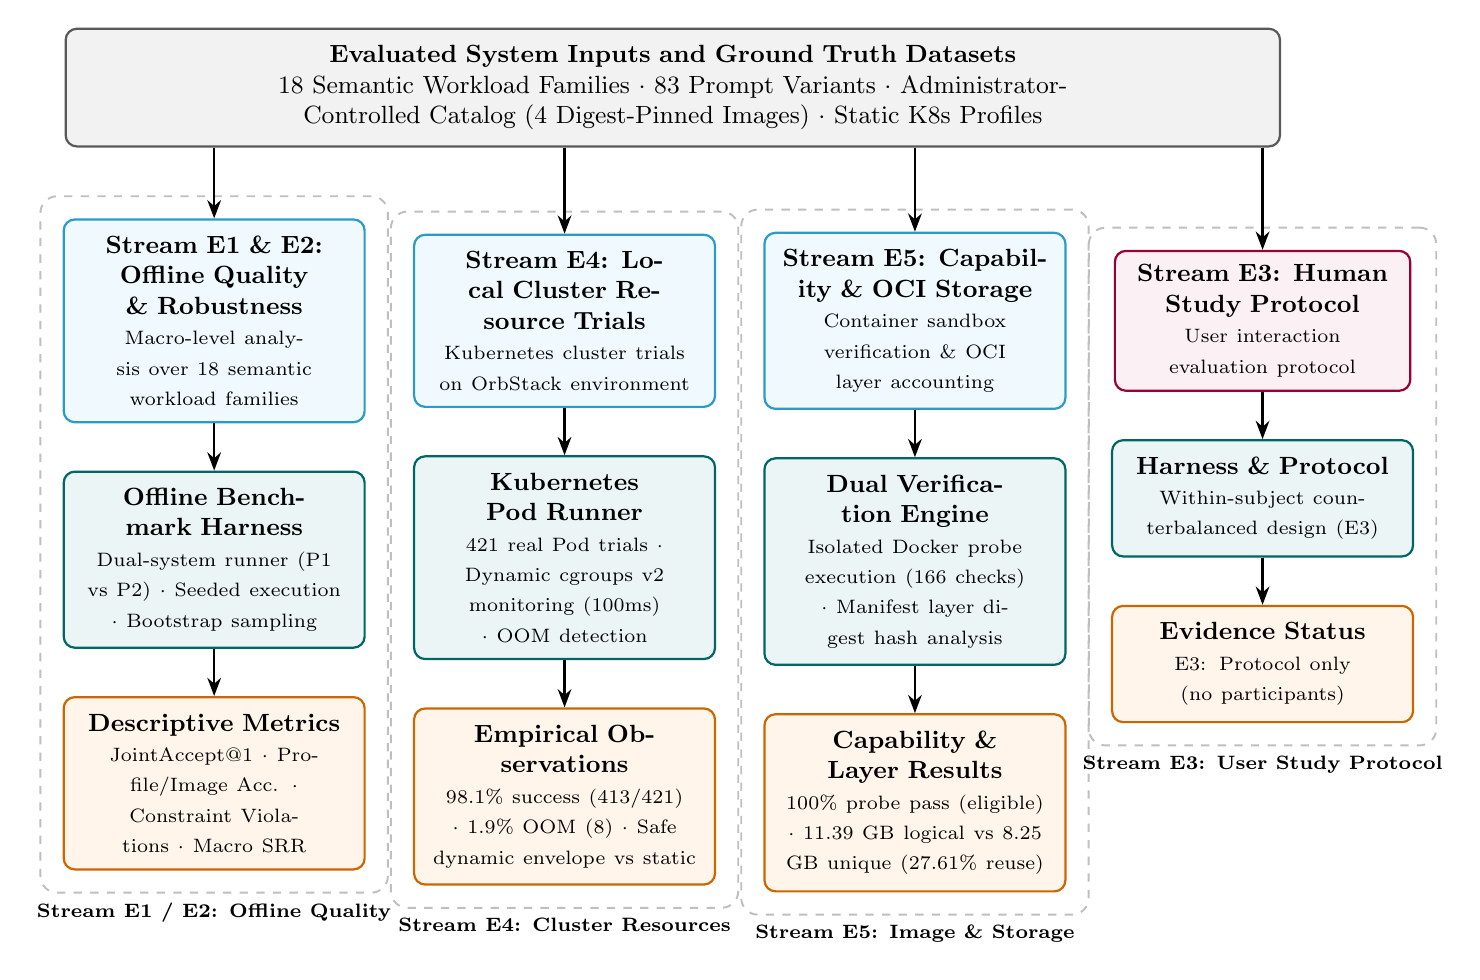
\begin{tikzpicture}[
    font=\small,
    >=Stealth,
    node distance=1.1cm and 0.8cm,
    box/.style={
        draw=blue!70!black,
        fill=blue!5,
        rounded corners=4pt,
        align=center,
        line width=0.8pt,
        inner sep=6pt,
        minimum height=0.9cm
    },
    stream/.style={
        box,
        draw=cyan!80!black,
        fill=cyan!6,
        text width=3.4cm
    },
    eval/.style={
        box,
        draw=teal!80!black,
        fill=teal!8,
        text width=3.4cm
    },
    metric/.style={
        box,
        draw=orange!80!black,
        fill=orange!8,
        text width=3.4cm
    },
    decision/.style={
        draw=purple!80!black,
        fill=purple!6,
        rounded corners=4pt,
        align=center,
        line width=0.8pt,
        inner sep=5pt,
        text width=3.4cm,
        minimum height=0.9cm
    },
    group/.style={
        draw=gray!50,
        dashed,
        rounded corners=6pt,
        line width=0.7pt,
        inner sep=8pt
    }
]

% Top Layer: Input & Target Scope
\node[box, text width=15cm, fill=gray!10, draw=gray!70!black] (input) {
    \textbf{Evaluated System Inputs and Ground Truth Datasets}\\
    18 Semantic Workload Families $\cdot$ 83 Prompt Variants $\cdot$ Administrator-Controlled Catalog (4 Digest-Pinned Images) $\cdot$ Static K8s Profiles
};

% Stream E1 & E2
\node[stream, below=0.9cm of input.south west, xshift=1.9cm] (e1_stream) {
    \textbf{Stream E1 \& E2: Offline Quality \& Robustness}\\
    \scriptsize Macro-level analysis over 18 semantic workload families
};
\node[eval, below=0.6cm of e1_stream] (e1_eval) {
    \textbf{Offline Benchmark Harness}\\
    \scriptsize Dual-system runner (P1 vs P2) $\cdot$ Seeded execution $\cdot$ Bootstrap sampling
};
\node[metric, below=0.6cm of e1_eval] (e1_metric) {
    \textbf{Descriptive Metrics}\\
    \scriptsize JointAccept@1 $\cdot$ Profile/Image Acc. $\cdot$ Constraint Violations $\cdot$ Macro SRR
};

% Stream E4
\node[stream, right=0.6cm of e1_stream] (e4_stream) {
    \textbf{Stream E4: Local Cluster Resource Trials}\\
    \scriptsize Kubernetes cluster trials on OrbStack environment
};
\node[eval, below=0.6cm of e4_stream] (e4_eval) {
    \textbf{Kubernetes Pod Runner}\\
    \scriptsize 421 real Pod trials $\cdot$ Dynamic cgroups v2 monitoring (100ms) $\cdot$ OOM detection
};
\node[metric, below=0.6cm of e4_eval] (e4_metric) {
    \textbf{Empirical Observations}\\
    \scriptsize 98.1\% success (413/421) $\cdot$ 1.9\% OOM (8) $\cdot$ Safe dynamic envelope vs static
};

% Stream E5
\node[stream, right=0.6cm of e4_stream] (e5_stream) {
    \textbf{Stream E5: Capability \& OCI Storage}\\
    \scriptsize Container sandbox verification \& OCI layer accounting
};
\node[eval, below=0.6cm of e5_stream] (e5_eval) {
    \textbf{Dual Verification Engine}\\
    \scriptsize Isolated Docker probe execution (166 checks) $\cdot$ Manifest layer digest hash analysis
};
\node[metric, below=0.6cm of e5_eval] (e5_metric) {
    \textbf{Capability \& Layer Results}\\
    \scriptsize 100\% probe pass (eligible) $\cdot$ 11.39 GB logical vs 8.25 GB unique (27.61\% reuse)
};

% Stream E3 (Supplementary / Protocols)
\node[decision, right=0.6cm of e5_stream] (aux_stream) {
    \textbf{Stream E3: Human Study Protocol}\\
    \scriptsize User interaction evaluation protocol
};
\node[eval, below=0.6cm of aux_stream] (aux_eval) {
    \textbf{Harness \& Protocol}\\
    \scriptsize Within-subject counterbalanced design (E3)
};
\node[metric, below=0.6cm of aux_eval] (aux_metric) {
    \textbf{Evidence Status}\\
    \scriptsize E3: Protocol only (no participants)
};

% Connections
\draw[->, line width=0.8pt] (input.south -| e1_stream.north) -- (e1_stream.north);
\draw[->, line width=0.8pt] (input.south -| e4_stream.north) -- (e4_stream.north);
\draw[->, line width=0.8pt] (input.south -| e5_stream.north) -- (e5_stream.north);
\draw[->, line width=0.8pt] (input.south -| aux_stream.north) -- (aux_stream.north);

\draw[->, line width=0.8pt] (e1_stream) -- (e1_eval);
\draw[->, line width=0.8pt] (e1_eval) -- (e1_metric);

\draw[->, line width=0.8pt] (e4_stream) -- (e4_eval);
\draw[->, line width=0.8pt] (e4_eval) -- (e4_metric);

\draw[->, line width=0.8pt] (e5_stream) -- (e5_eval);
\draw[->, line width=0.8pt] (e5_eval) -- (e5_metric);

\draw[->, line width=0.8pt] (aux_stream) -- (aux_eval);
\draw[->, line width=0.8pt] (aux_eval) -- (aux_metric);

% Group background
\begin{scope}[on background layer]
    \node[group, fit=(e1_stream)(e1_metric), label=below:{\scriptsize \textbf{Stream E1 / E2: Offline Quality}}] {};
    \node[group, fit=(e4_stream)(e4_metric), label=below:{\scriptsize \textbf{Stream E4: Cluster Resources}}] {};
    \node[group, fit=(e5_stream)(e5_metric), label=below:{\scriptsize \textbf{Stream E5: Image \& Storage}}] {};
    \node[group, fit=(aux_stream)(aux_metric), label=below:{\scriptsize \textbf{Stream E3: User Study Protocol}}] {};
\end{scope}

\end{tikzpicture}
\end{document}
